Auf Grundlage der zuvor genannten Messvoraussetzungen konnte die Roboter-Gesten-Anwen-\\dung verschiedenen Tests unterzogen und deren Ergebnisse ausgewertet werden. Zur Durchführung der Tests wurde die Roboter-Gesten-Anwendung mit zusätzlichen \quoteMark{*\_MEASUREMENT}-Flags, zu denen die Flags \quoteMark{GESTURE\_MEASUREMENT}, \quoteMark{COMMUNICATION\_MEASU-\\REMENT} und \quoteMark{POSITION\_MEASUREMENT} zählen, kompiliert um ausführliche Statistikdaten für den jeweils durchgeführten Testfall zu erhalten. Die durchgeführten Tests reichen hierbei von Latenztests der Gestenerkennung mittels der Azure Kinect über Latenztests der Kommunikation mittels ROS und der direkten Kommunikation mit dem \quoteMark{WidowX 200}-Lernroboter bis hin zu der Genauigkeit der anzufahrenden Zielpositionen. Die erhobenen statistischen Daten wurden analysiert und werden nachfolgend mittels Diagrammen veranschaulicht und kritisch hinterfragt.

% Implementierung: Roboter wählt seine eigene Bahn
% Bewegen durch Gesten in beliebigen Koordinatensystemen mit unterschiedlichen Orientierungen

% Wie lange benötige ich für das Teachen mittels Gesten? Ist es ein vertretbarer Aufwand? Was ist ein vertretbarer Aufwand?

% Hierfür wurde darauf geeinigt, dass die Bewegungsabläufe des Roboters auch nachträglich nachbearbeitet werden können.

% Wünschenswert, die Bewegungen können jedoch aber im nachhinein auch nachträglich nachbearbeitet werden. Wenige mm wären ideal, aber wenige cm würden auch genügen.

% ------------

% Azure Kinect: Belichtungszeit: 1,6 ms bis zu 20,3 ms (https://docs.microsoft.com/en-us/azure/kinect-dk/hardware-specification) -> TODO: Passive IR einschalten?
% Realsens: Belichtungszeit: 900 ns (https://www.imveurope.com/press-releases/intel-realsense-lidar-depth-camera-l515) (https://softei.com/framos-claims-hi-res-intel-realsense-lidar-depth-camera-is-worlds-smallest/) (https://venturebeat.com/2019/12/11/intels-new-realsense-camera-packs-a-lidar-sensor-for-enhanced-depth-perception/) -> Distanz?
% https://www.intelrealsense.com/compare-depth-cameras/
% https://www.intelrealsense.com/depth-camera-d435/

% https://docs.microsoft.com/en-us/windows/mixed-reality/ISSCC-2018



%----------------

% https://feedback.azure.com/forums/920053-azure-kinect-dk/suggestions/38129473-body-tracking-without-cudnn
% https://feedback.azure.com/forums/920053-azure-kinect-dk/suggestions/39945454-legacy-body-tracking-like-kinect-v2
% https://github.com/microsoft/Azure-Kinect-Sensor-SDK/issues/1080



%-----------
% konkrete Aussage zur Performanz, Stabilität, Modularität, Hohe Skalierbarkeit,
% Erweiterbarkeit

% Erfahrungen

% Mögliche Prognosen

% Limitierungen

% Entwicklungswerkzeuge


% --------------

% weiche Echtzeitfähigkeit
% Durchsatz, Latenzen, ...

% Die Gestensteuerung des WidowX 200, welches auf dem für diese Arbeit erstellten Roboter-Gesten-Framework basiert und als Basis für andere gestengesteuerte Roboter dienen kann, wird auf die Ergonomie, Echtzeitfähigkeit, Genauigkeit der Gestenerkennung und Genauigkeit der Zielpositionen hin überprüft. Zudem wird ROS 1 auf die Netzwerklatenz hin überprüft um darauf basierend eine Einschätzung zu gegeben ob sich ROS 1 für echtzeitfähige Systeme eignet.

\section{Latenz der Gestenerkennung}
Zum Testen der Latenz der Gestenerkennung wurde das Azure Kinect Body Tracking SDK im CPU-Modus anstatt mit der Grafikkartenbeschleunigung gestartet. Dies war notwendig, da eine Grafikkarte von AMD statt einer Nvidia Grafikkarte im Testsystem eingesetzt wird. Zudem kann hiermit der kleinste gemeinsame Nenner der im Umlauf befindlicher Systeme widergespiegelt werden, welche keine propritären Features, wie z.B. CUDA, von Nvidia Grafikkarten verwenden. Als alternative und platformunabhängige Programmierschnittstelle zu CUDA wäre hier z.B. OpenCL oder Vulkan anzumerken \cite{vulkan_api_2020}. Die Latenz der Gestenerkennung beinhaltet die Zeit vom Aussenden des Infrarot-Lichtimpuls bis zum Empfang und Absorption des Lichtimpuls bis hin zur Latenz über das \quoteMark{USB 3.0}-Kabel und der Verarbietung der Daten durch das Azure Kinect Body Tracking SDK. Zum Testen der Latenz der Gestenerkennung wurde die Roboter-Gesten-Anwendung und deren Abhängigkeiten mittels der Flags \quoteMark{MEASUREMENT} und \quoteMark{GESTURE\_MEASUREMENT}, welche im Anhang \ref{appendix1.2:Installation_und_Konfiguration_der_Pakete} aufgezeigt werden, kompiliert. Die Datei \quoteMark{Messung der Gestenerkennung.csv}, welche bei der Durchführung des Tests von der Roboter-Gesten-Anwendung erstellt wurde, ist auf der CD/ISO im Verzeichnis \quoteMark{Testdaten/} zu finden.

\begin{figure}[htb]
	\centering
	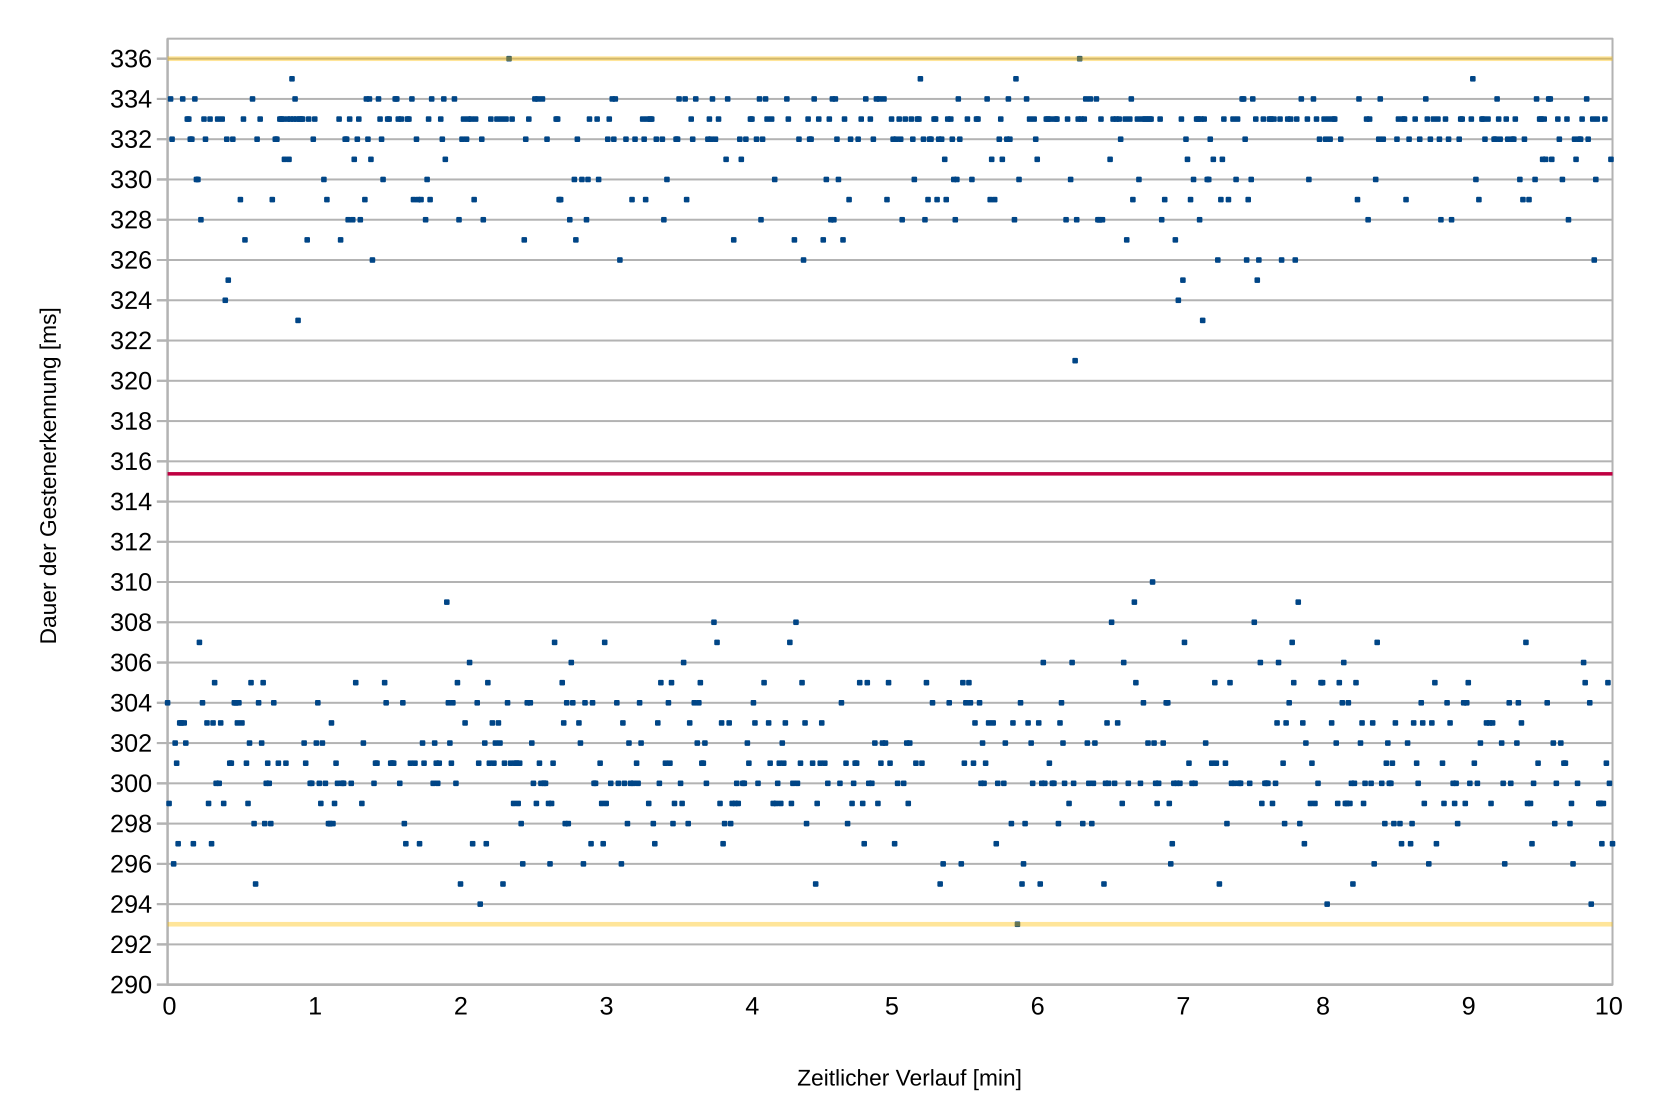
\includegraphics[width=1.04\textwidth]{images/ergebnisse/dauer_der_gestenerkennung_verlauf}
	\caption[Zeitlicher Latenzverlauf der Gestenerkennung der Azure Kinect]{Zeitlicher Latenzverlauf der Gestenerkennung der Azure Kinect\\Quelle: Eigene Ausarbeitung}
	\label{fig:measurement_gesture_recognition_azure_kinect}
\end{figure}
\FloatBarrier

In Abbildung \ref{fig:measurement_gesture_recognition_azure_kinect} ist zu sehen, dass der Mittelwert der Gestenerkennungsdauer, welcher durch die hellrote Linie visualisiert wird, in Richtung \num{326,29} ms tendiert. Die minimale Dauer der Gestenerkennung, welche durch die untere orange Linie visualisiert wird, beträgt \num{291} ms. Die maximale Dauer der Gestenerkennung, welche durch die obere orange Linie visualisiert wird, beträgt hingegen \num{366} ms. Die violette Linie stellt die Tendenz der Gestenerkennungsdauer dar, welche jedoch gleich zu bleiben scheint. Anzumerken ist, dass die Gestenerkennungsdauer sich im Durchschnitt stabil im Bereich zwischen \num{314,02} ms und \num{338,55} ms bewegt. Die annähernd gleich bleibende Gestenerkennungsdauer kann auf das DNN des Azure Kinect Body Tracking SDKs und den eingesetzten Prozess-Scheduler zurückgeführt werden. Eine nichtdeterministische Berechnung würde hierbei vermehrt Spikes und unvorhersagbarere Änderungen bei der Gestenerkennungsdauer bewirken. Nichtsdestotrotz liegen diese Werte weit über den 50 ms, welches für ein Teach Pendant empfohlen wird \cite[55]{prassler_advances_2004}. Zudem ist eine Verzögerung der Gestenerkennung bei über 100 ms für die bedienende Person bereits deutlich spürbar \cite{miller_response_1968}.

\section{Latenz der Roboter-Kommunikation mit und ohne ROS-Anbindung}
Für diesen Testfall wurde die Roboter-Gesten-Anwendung und deren Abhängigkeiten mittels der Flags \quoteMark{MEASUREMENT} und \quoteMark{COMMUNICATION\_MEASUREMENT}, welche im Anhang \ref{appendix1.2:Installation_und_Konfiguration_der_Pakete} aufgezeigt werden, kompiliert.
\textcolor{red}{TODO:\\
Praxistest mit zusätzlicher Gestenerkennung oder ohne?\\
WidowX 200\\
Verschiedene Netzwerkkonstellationen simulieren? % aus dem Sicherheitsaspekt sollte für ROS 1 ein eigens für den Roboter abgeschottenes Netzwerk verwendet -> dadurch meisten weniger Latenzen, weil weniger über ROS übertragen wird?
% http://wiki.ros.org/Topics
% Topic statistics
}

\begin{figure}[htb]
	\centering
	\includegraphics[width=1.04\textwidth]{images/ergebnisse/Messung_der_direkten_Kommunikation}
	\caption[Zeitlicher Latenzverlauf der direkten Kommunikation des \quoteMark{WidowX 200}-Lernroboters]{Zeitlicher Latenzverlauf der direkten Kommunikation des \quoteMark{WidowX 200}-Lernroboters\\Quelle: Eigene Ausarbeitung}
	\label{fig:measurement_robot_direct_communication}
\end{figure}
\FloatBarrier

\begin{figure}[htb]
	\centering
	\includegraphics[width=1.04\textwidth]{images/ergebnisse/Messung_der_ROS_Kommunikation_App_und_keine_Netzwerksimulation}
	\caption[Zeitlicher Latenzverlauf der ROS-Kommunikation des \quoteMark{WidowX 200}-Lernroboters (ohne Netzwerksimulation)]{Zeitlicher Latenzverlauf der ROS-Kommunikation des \quoteMark{WidowX 200}-Lernroboters (ohne Netzwerksimulation)\\Quelle: Eigene Ausarbeitung}
	\label{fig:measurement_robot_ros_without_network_simulation}
\end{figure}
\FloatBarrier

\begin{figure}[htb]
	\centering
	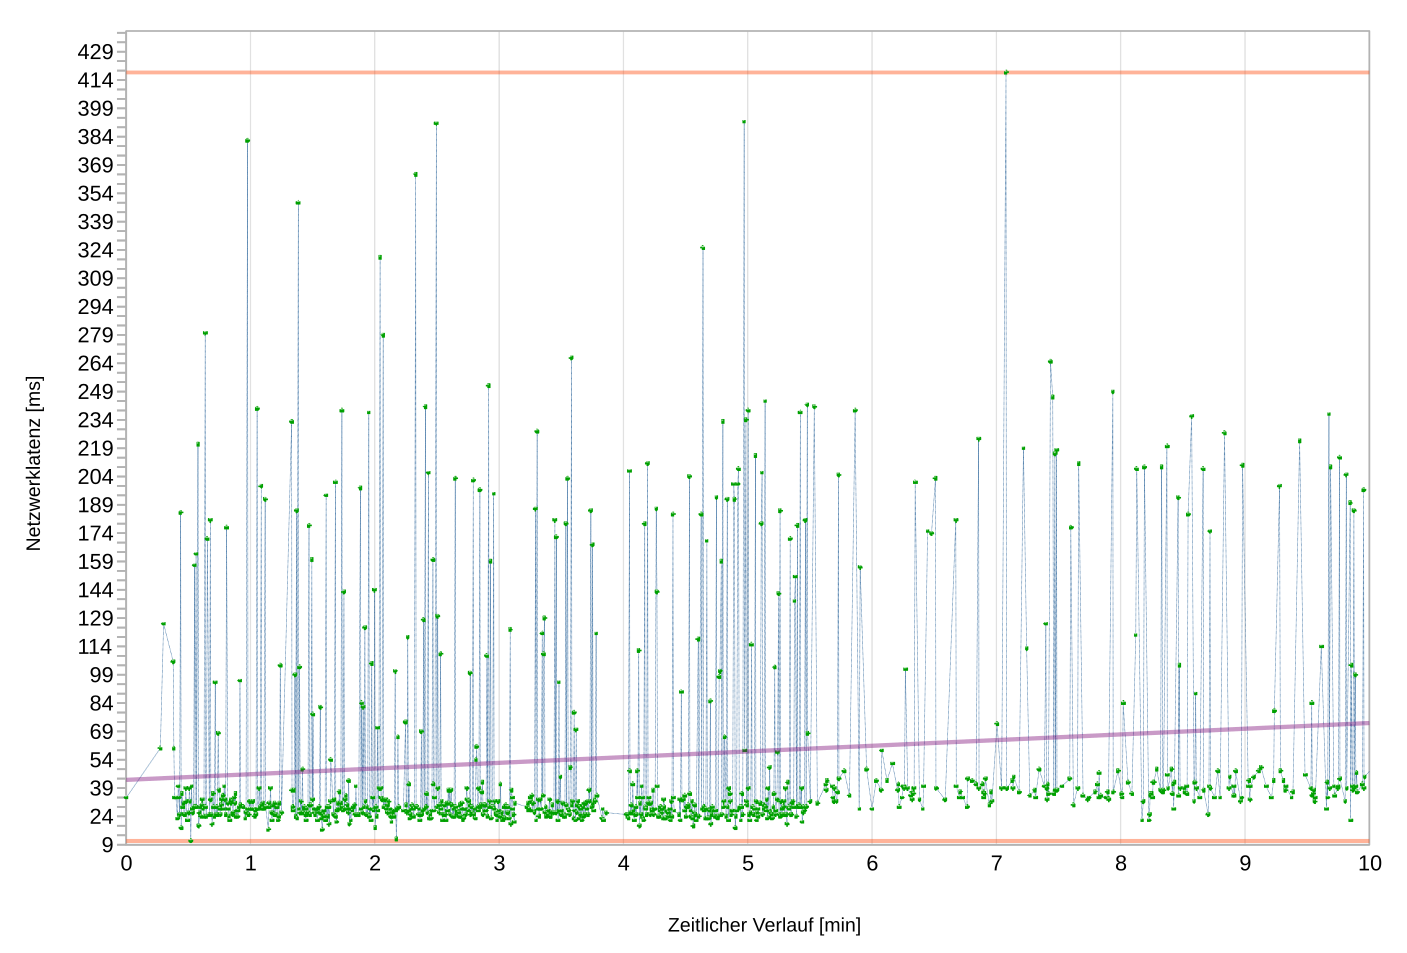
\includegraphics[width=1.04\textwidth]{images/ergebnisse/ROS_App_und_mit_Netzwerksimulation}
	\caption[Zeitlicher Latenzverlauf der ROS-Kommunikation des \quoteMark{WidowX 200}-Lernroboters (mit Netzwerksimulation, geringe Netzwerkauslastung)]{Zeitlicher Latenzverlauf der ROS-Kommunikation des \quoteMark{WidowX 200}-Lernroboters (mit Netzwerksimulation, geringe Netzwerkauslastung)\\Quelle: Eigene Ausarbeitung}
	\label{fig:measurement_robot_ros_with_network_simulation_low_network_traffic}
\end{figure}
\FloatBarrier

\begin{figure}[htb]
	\centering
	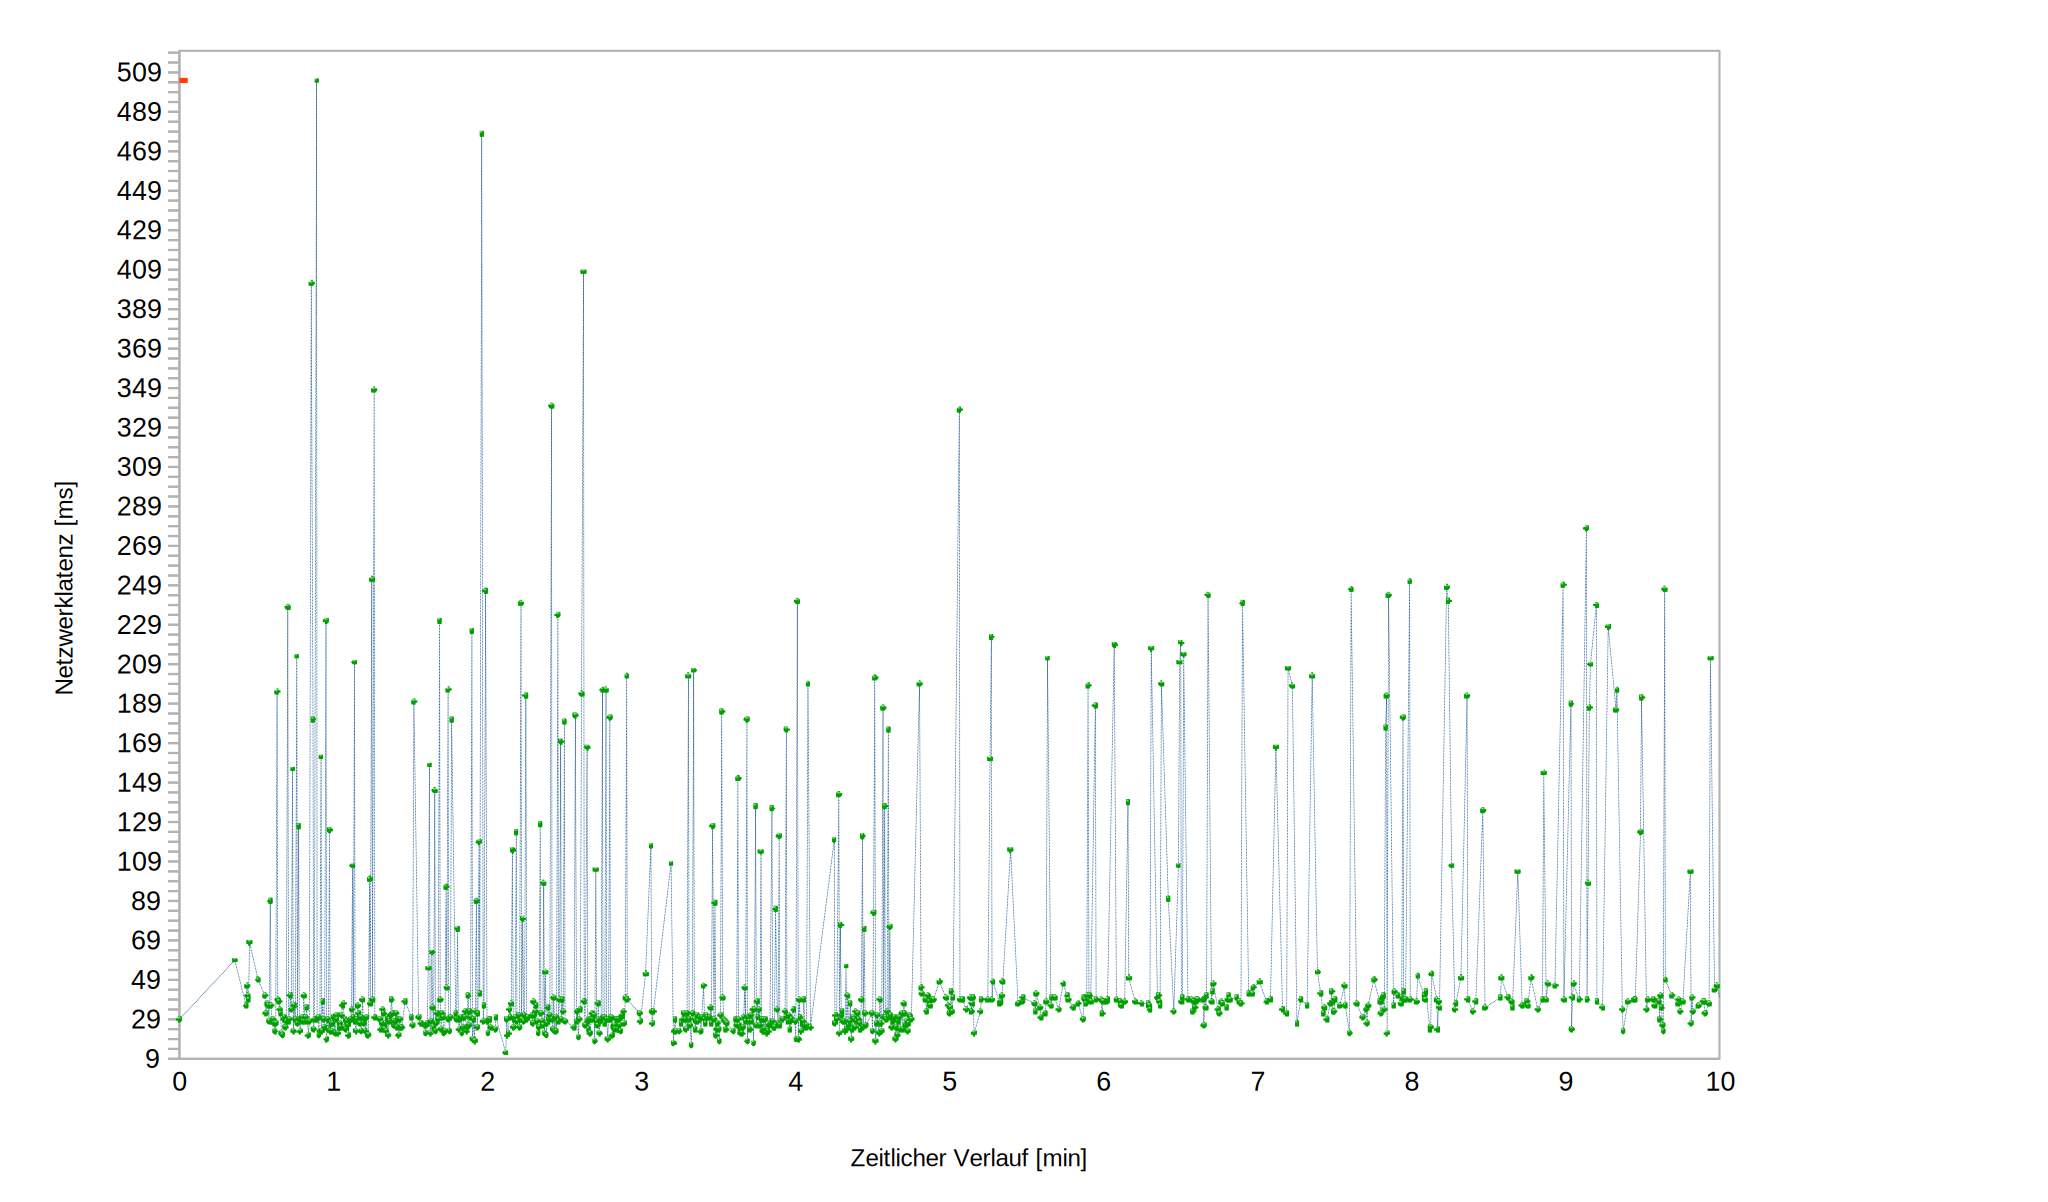
\includegraphics[width=1.04\textwidth]{images/ergebnisse/ROS_App_mit_Netzwerksimulation_und_hohe_Auslastung}
	\caption[Zeitlicher Latenzverlauf der ROS-Kommunikation des \quoteMark{WidowX 200}-Lernroboters (mit Netzwerksimulation, hohe Netzwerkauslastung)]{Zeitlicher Latenzverlauf der ROS-Kommunikation des \quoteMark{WidowX 200}-Lernroboters (mit Netzwerksimulation, hohe Netzwerkauslastung)\\Quelle: Eigene Ausarbeitung}
	\label{fig:measurement_robot_ros_with_network_simulation_high_network_traffic}
\end{figure}
\FloatBarrier

% catkin build -DCMAKE_BUILD_TYPE=Release --cmake-args -DCMAKE_CXX_FLAGS="-DCOMMUNICATION_MEASUREMENT -DMEASUREMENT"
% interbotix_communication_measurement.csv

% für ROS: ein Testnetzwerk aufbauen unterschiedliche Latenzen testen
% Best Case: keine Latenzen
% Worst Case: Übertragen von größeren Datenmengen über ROS (z.B. Kamerabilder, …)

% vom Übertragen des Befehls an die Steuerungseinheit bis der Roboter die Bewegung durchführt
%vom Übertragen des Befehls über TCP/IP bis zur Steuerungseinheit
%vom Durchführen der Geste bis zum erfolgreichen Erkennen von unterschiedlichen Gesten. Unterschiedliche Gesten können mitunter z.T. mehr oder weniger Zeit beanspruchen je nach Komplexität der Geste.


\section{Genauigkeit der Zielpositionen}
Zur Genauigkeitsmessung der Zielpositionen werden diese im Simulator Gazebo durchgeführt. In der Simulationsumgebung wurde ein virtueller Raum erschaffen, in welchem die Zielpositionen bereits genau vordefiniert sind. Die ermittelten Positionen können daraufhin mit den exakten Positionen verglichen werden um so genaue Differenzen bestimmen zu können.

Für diesen Testfall wurde die Roboter-Gesten-Anwendung und deren Abhängigkeiten mittels der Flags \quoteMark{MEASUREMENT} und \quoteMark{POSITION\_MEASUREMENT}, welche im Anhang \ref{appendix1.2:Installation_und_Konfiguration_der_Pakete} aufgezeigt werden, kompiliert.

\textcolor{red}{TODO}

%Im Vergleich zu einer anderen Eingabemethode%\\
%PS3-Controller: https://www.trossenrobotics.com/widowx-200-robot-arm.aspx

% Wie genau kommt man ans gewünschte Ziel? (Einheit: mm)
% Wie viele Korrekturen braucht ein Proband um am nächsten ans gewünschte Ziel zu kommen?

% In einer realen Umgebung nur mit Ungenauigkeiten messbar
%In einer Simulationsumgebung (z.B. Gazebo) kann die Distanz genau und automatisiert gemessen werden
%Visualisierung:
%  *Diagramme
%  *    Mittelwert, die Standardabweichung, Varianz, ...

\begin{figure}[htb]
	\centering
	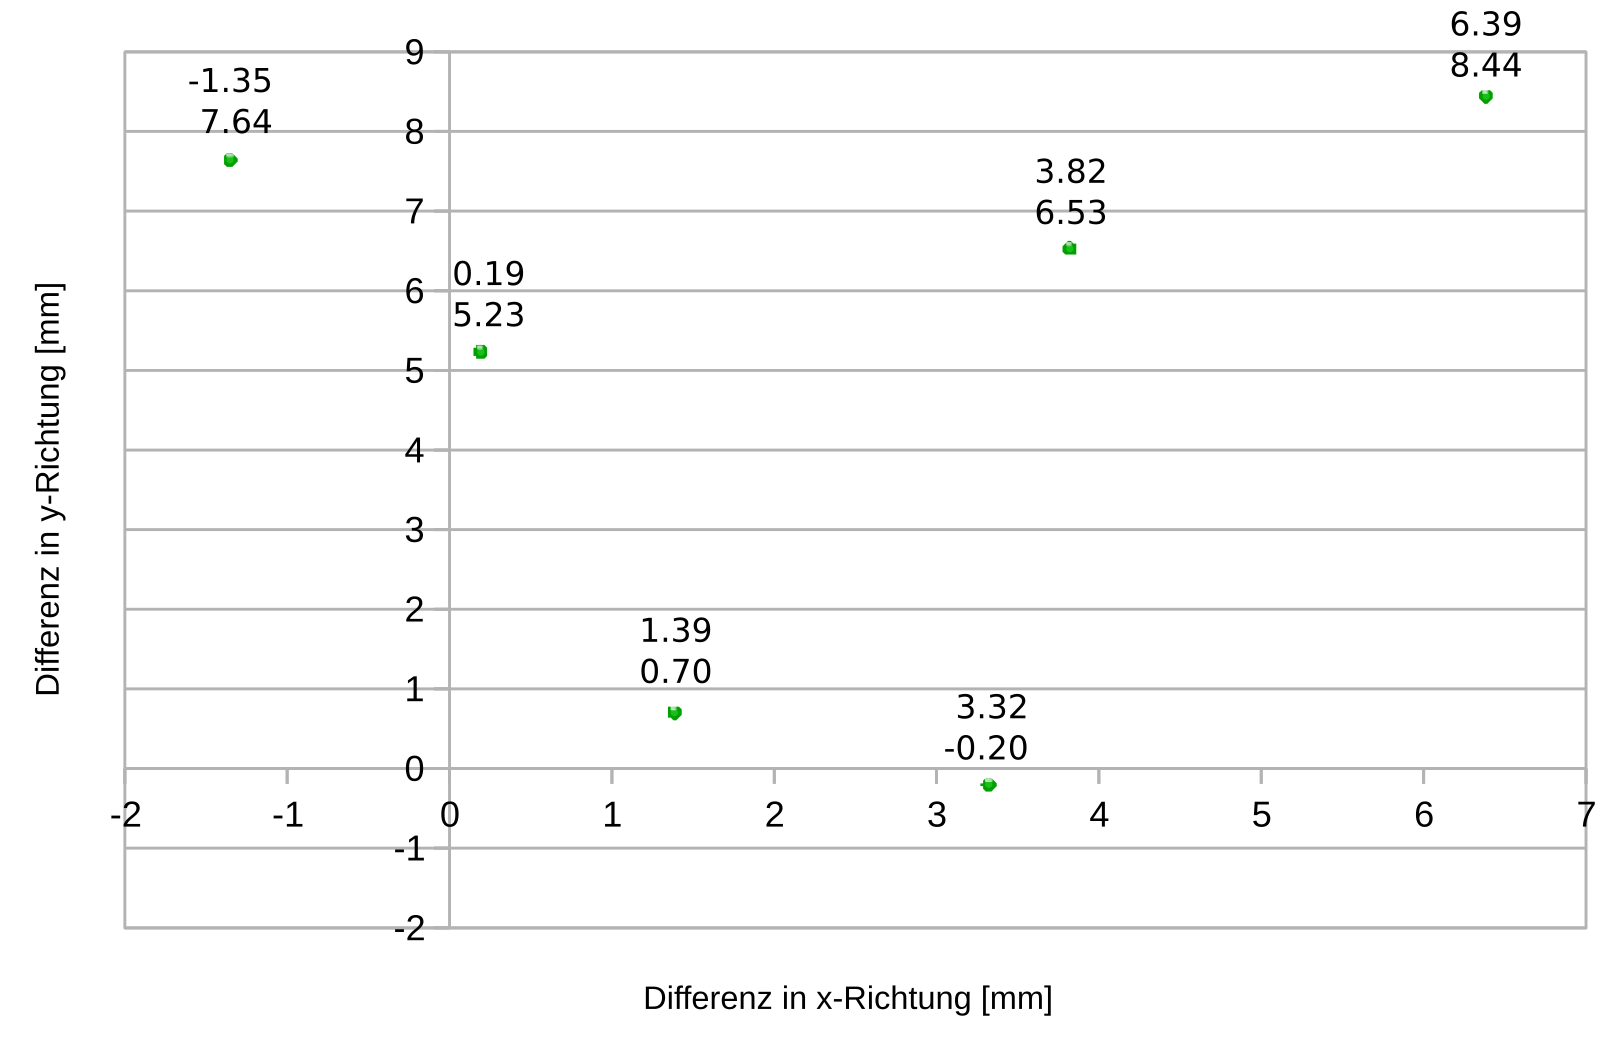
\includegraphics[width=0.88\textwidth]{images/ergebnisse/Differenzen_beim_Teachen_mit_Gesten}
	\caption[Positionsdifferenzen beim Teachen mit der Roboter-Gesten-Anwendung]{Positionsdifferenzen beim Teachen mit der Roboter-Gesten-Anwendung\\Quelle: Eigene Ausarbeitung}
	\label{fig:measurement_teaching_positions}
\end{figure}
\FloatBarrier

\begin{figure}[htb]
	\centering
	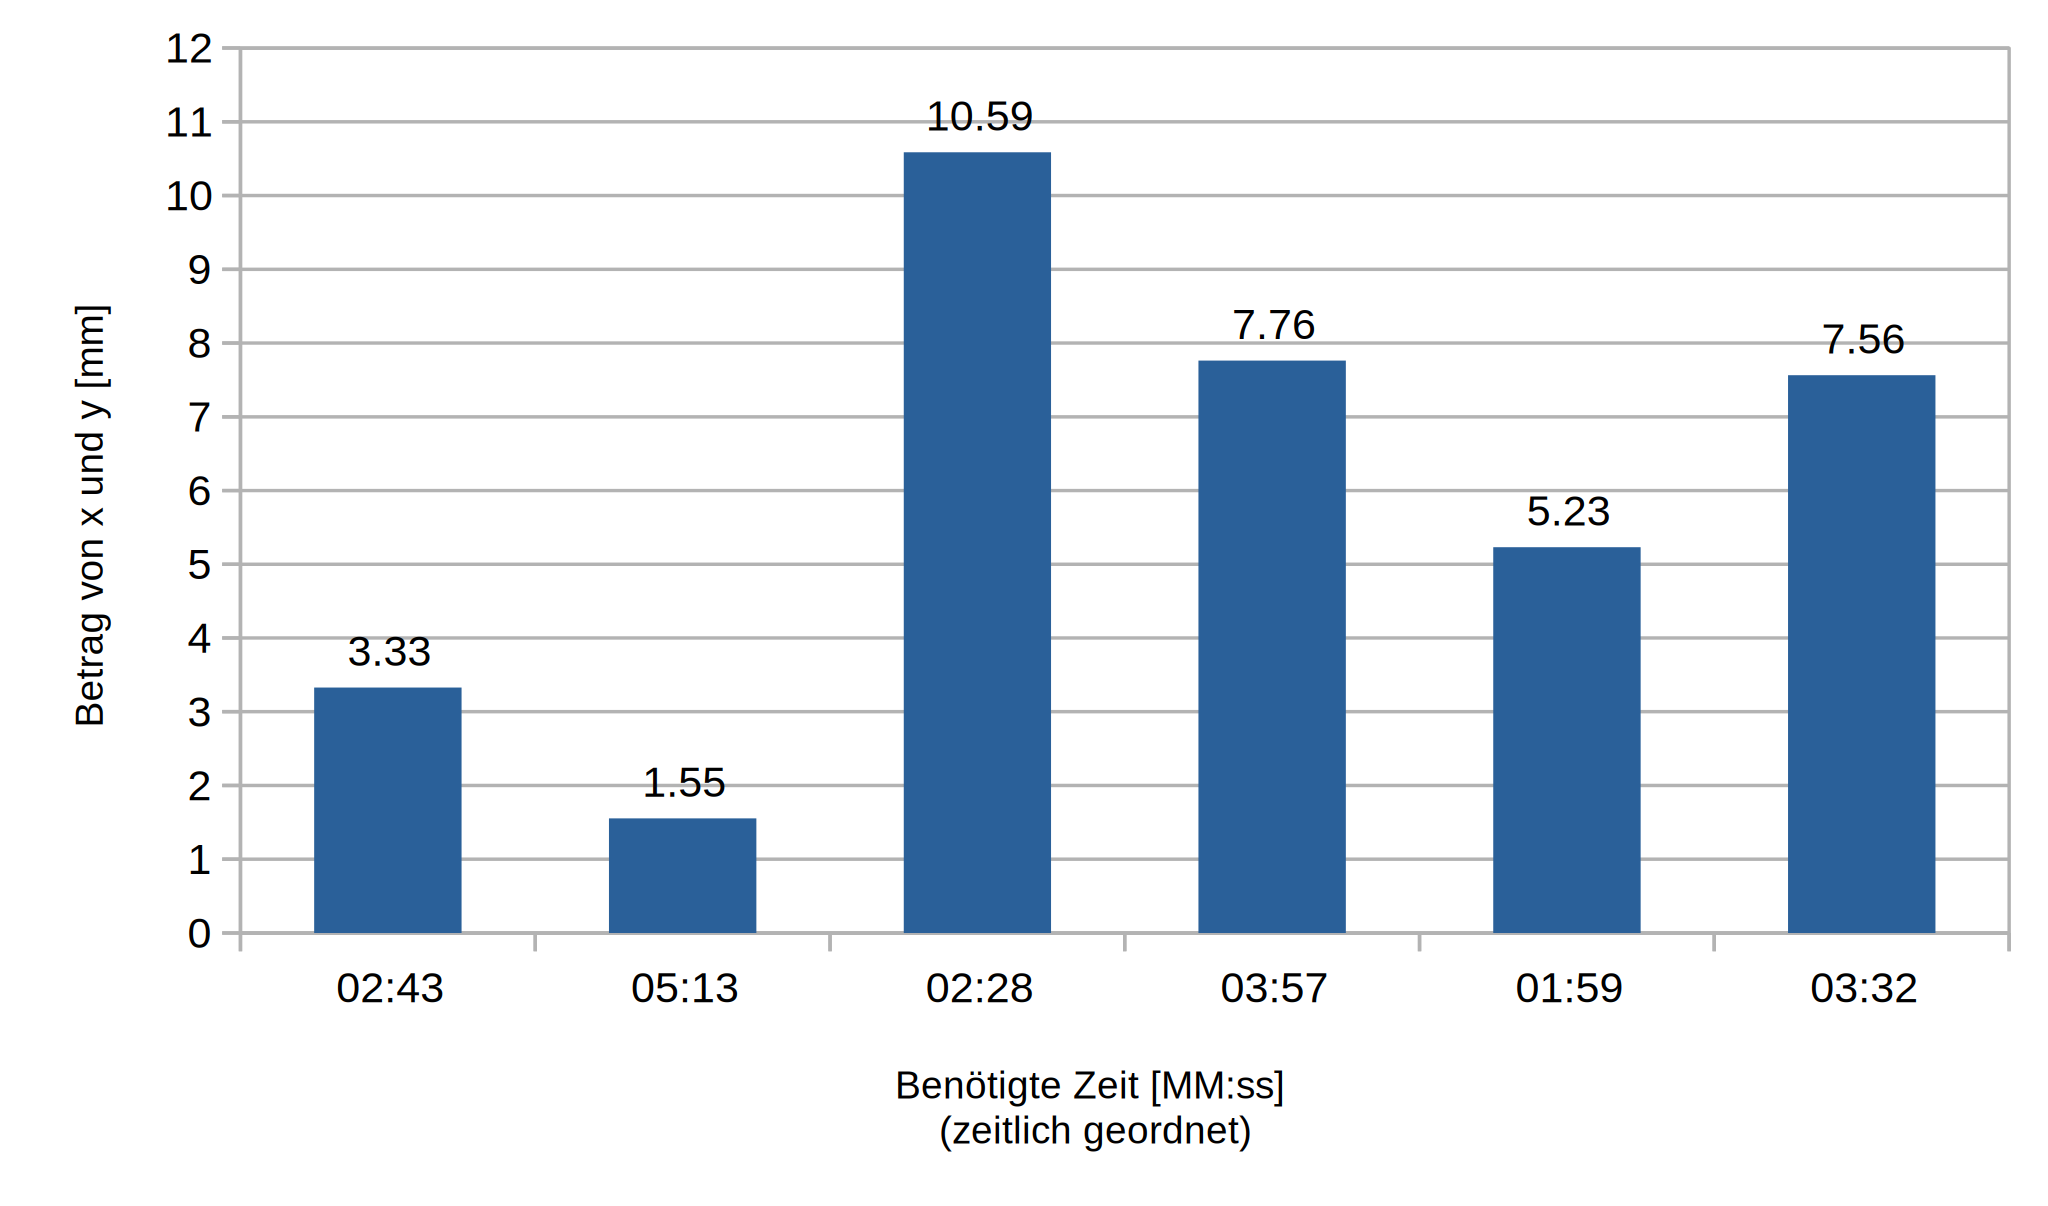
\includegraphics[width=0.88\textwidth]{images/ergebnisse/Betrag_der_Fehlerquadrate}
	\caption[Betrag der Fehlerquadrate beim Teachen mit der Roboter-Gesten-Anwendung]{Betrag der Fehlerquadrate beim Teachen mit der Roboter-Gesten-Anwendung\\Quelle: Eigene Ausarbeitung}
	\label{fig:measurement_teaching_positions}
\end{figure}
\FloatBarrier

\section{Genauigkeit der Gestenerkennung}
% Wie viele Versuche benötigt ein Proband bis seine Gesten erkannt werden?

% \section{Ergonomie \& User Experience}
% Verbessert dieser Ansatz die Ergonomie des Teachen in eine positive Richtung?
% Ist es angenehmer diese NUI-Methode zu verwenden als ein herkömmliches Teach Pendant?
% Kann ich über eine längere Zeitspanne, wie z.B. 30 Minuten, einen Roboter teachen?
% Wie schnell bin ich erschöpft im Gegensatz zu einem herkömmlichen Teach Pendant?
% Wie schnell erlernt man die Gesten?
% Wie einprägsam sind die Gesten?
% Sind die Gesten gut geeignet um einen Roboter zu steuern oder sind diese zu schwammig oder zu ähnlich und werden daher auch oft verwechselt?
%   * Können diese im besten Fall nur schwer unbeabsichtigt durchgeführt werden und fälschlicherweise nicht z.B. als kulturelle Geste erkannt werden?
%   * Gibt es wenige Überschneidungen mit bereits definierten Gesten, sodass diese nicht unbeabsichtigt durchgeführt werden können?
%   * Sind diese leicht anzuwenden, sodass das System die Geste im besten Fall beim ersten Mal erkennt?

% Erkennungsrate der Gestenerkennung

\textcolor{red}{TODO:\\
Wie gut ist das System einsetzbar? UX\\
Bewertung der Ergonomie über längere Zeitdauer (sehr subjektiv, jedoch aber versuchen die Ergebnisse auf die Allgemeinheit zu bezienen)\\
Während dem Teachen bewegt man sich oft um zu sehen ob der Endeffektor an der richtigen Stelle ist. Mit einer fest angebrachten Azure Kinect ist es daher schwer den eigenen Blickwinkel zu ändern\\
reflexartige und unbeabsichtigte Bewegungen\\
Beim Teachen steht man normalerweise um den Roboter ordnungsgemäß und vollständig sehen zu können
% siehe 3.4.3 Auswahl anhand der Ergonomie
}

% muss nicht auf die Körpergröße eingestellt werden, da der Field of View sehr groß ist

% Kann ich über eine längere Zeitspanne, wie z.B. 30 Minuten, einen Roboter teachen? Wie schnell bin ich erschöpft im Gegensatz zu einem herkömmlichen Teachpendant? Wie schnell lernt man die Gesten? Sind die Gesten gut geeignet um einen Roboter zu steuern oder sind diese zu schwammig oder zu ähnlich und werden daher auch oft verwechselt?
